\documentclass{article}
\usepackage[portuguese]{babel}
\usepackage{graphicx}
\usepackage{listings}
\usepackage[utf8]{inputenc}
\usepackage{listings}
\lstset{language=Java, breaklines=true, basicstyle=\footnotesize} % Especificar Haskell, mudar de linha quando acabar espaço, diminuir tamanho da letra.
\usepackage{indentfirst} %Identação nos parágrafos iniciais
%\graphicspath{ {/home/jessica/Documentos/Engineer/Geocaching-Java} }

\renewcommand{\baselinestretch}{2}
%\author{no realizado por :P}
\title{Geocaching POO}
\date{Junho 2015}


\begin{document}
  \begin{titlepage}

\newcommand{\HRule}{\rule{\linewidth}{0.5mm}} % Defines a new command for the horizontal lines, change thickness here

\center % Center everything on the page

\textsc{\LARGE Universidade do Minho}\\[1.5cm] % Name of your university/college
\textsc{\Large LEI}\\[0.5cm] % Major heading such as course name
\textsc{\large Programação Orientada aos Objetos}\\[0.5cm] % Minor heading such as course title

\HRule \\[0.4cm]
{ \huge \bfseries Geocaching}\\[0.4cm] % Title of your document
\HRule \\[1.5cm]

\begin{figure}[!htb]
\minipage{0.31\textwidth}
  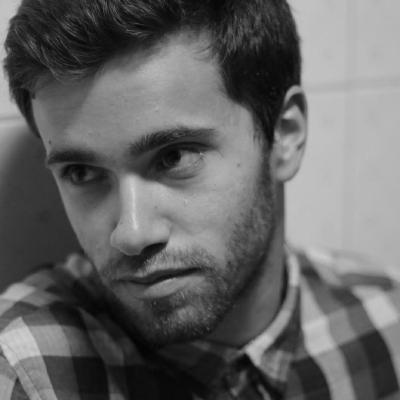
\includegraphics[width=\linewidth]{adelino.jpg}
  \caption*{João Costa A70563}\label{fig:awesome_image1}
\endminipage\hfill
\minipage{0.31\textwidth}
  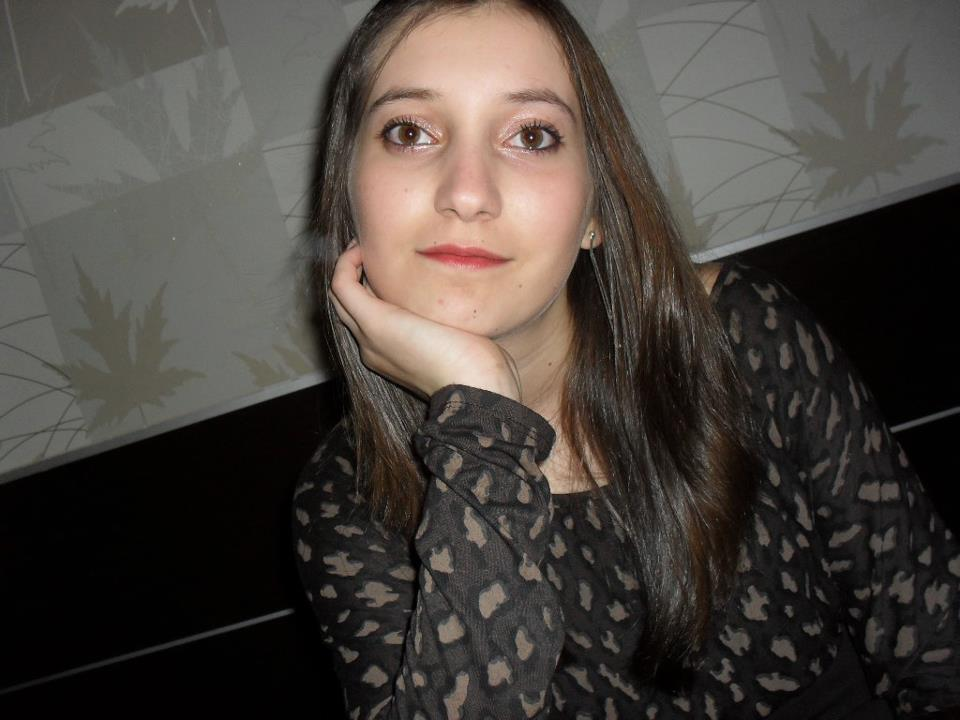
\includegraphics[width=\linewidth]{jessica0.jpg}
  \caption*{Jéssica Pereira A70563}\label{fig:awesome_image2}
\endminipage\hfill
\minipage{0.29\textwidth}%
  
\includegraphics[width=\linewidth]{martinho.jpg}
  \caption{Martinho Aragão A72205}
\endminipage
\end{figure}

{\large \today}\\[3cm] % Date, change the \today to a set date if you want to be precise

%\includegraphics[width=0.30\textwidth]{UM-EENG.jpg}\\[1cm] % Include a department/university logo - this will require the graphicx package

\vfill % Fill the rest of the page with whitespace

\end{titlepage}

\tableofcontents

\pagebreak

\section{Introdução}

\quad
Este trabalho sobre o conceito de Geocaching conhecido nas redes sociais: pretendemos simular
e registar atividades e descobrimentos de caches. Para isso foi necessário modularizar e fazer
as devidas abstrações na preparação para o trabalho, pois quanto mais abstrações forem criadas
mais independentes os módulos serão, podendo depois usar a composição entre estas classes e
fornecendo uma melhor compreensão do código e tratamento da informação.
\par
É necessário o estudo e concepção das classes necessárias, estruturas de dados, métodos
respetivos, variáveis de instância e de classe necessárias, imagina a dependência entre
as classes (composição) e definir uma hierarquia (nomeadamente criando uma super
class para as Caches).
\par Para além de criar classes abstratas, também é necessário guardar todos os dados relativos
às Caches e aos Utilizadores para poder criar métodos eficientes relativos ao tratamento
destes.
\par De entre os requesitos básicos também serão implementados os Eventos, com a simulação
da metereologia e cálculo de distâncias entre caches dados duas coordenadas (coordenadas
iniciais e as coordenadas da cache). Estes dois últimos pontos serão implementados também
em toda a descoberta de Caches/Actividades e não somente no decorrer de Eventos pois serão
úteis nomeadamente para o cálculo de pontuações.
\pagebreak

%Na introdução foram ditos os objetivos. :P

\section{Modularização - Classes criadas}

\quad Decidimos apenas criar 4 tipos de Caches visto a Cache-Evento nao fazer sentido quando temos uma classe que simula eventos, e a Cache Virtual ...
\par Guardamos todos os users e todas as caches criadas numa base de dados.
\par Para classes que usam estruturas do tipo set criamos vários comparadores úteis para diferentes tipos de ordenação a diferentes classes.
\par Inicialmente tinhamos uma classe chamada 'Server' que acabamos por eliminar pois esta baseia-se na classe GeocachingPOO. A ideia era na classe Server ter acesso a toda a informação, sendo esta apenas acessível aos Admins, mas no próprio GeocachingPOO temos a opção de fazer login como Admin, simplificando e colocando tudo numa classe.
\par Temos hierarquia quanto às caches e quanto aos users.
\par Temos Estatísticas globais, anuais e mensais.
\\
%adicionar imagem do trello final do diagrama
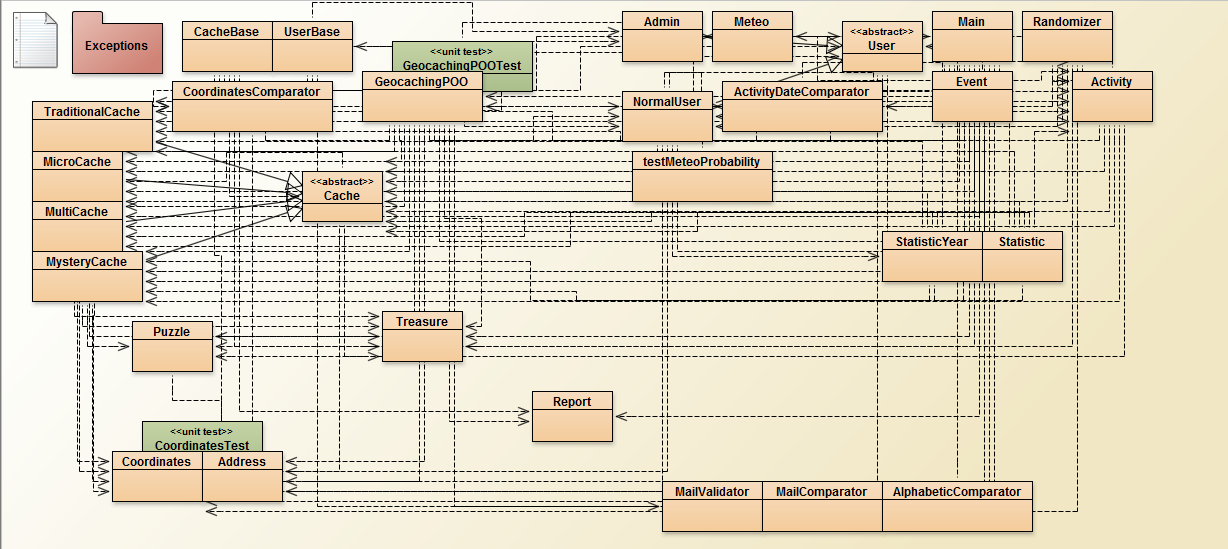
\includegraphics[height=8\baselineskip,natwidth=369,natheight=430]{Diagrama.PNG}

\pagebreak
\section{Bases de dados}

\subsection{CacheBase}
\par Antes de implementarmos a classe \textbf{CacheBase} reflectimos que características únicas teria cada cache para a
diferenciar de todas as outras.
\par Cada cache tem coordenadas únicas, não sendo possível criar uma cache em coordenadas onde já existe uma cache,
independentemente do tipo de cache, isto levou-nos a implementar um \textbf{TreeMap} para mapear coordenadas a
IDs de cache.
\par Para guardar as caches utilizamos um \textbf{ArrayList} visto que sabendo o ID de uma cache é bastante fácil encontrá-lo
nesta estrutura pois para um dado valor de ID sabemos que a Cache, caso exista, estará no indíce de valor igual a (ID - 1).
\par Portanto a implementação das variáveis de instância de \textbf{CacheBase} é a seguinte:
\begin{lstlisting}[language=Java]
/* ArrayList com as caches */
private ArrayList<Cache> caches;
/* Mapeamento entre e-mails e IDs */
private TreeMap<Coordinates, Double> coords;
\end{lstlisting}

\par Como é necessário um dado Utilizador poder ver as caches que criou utilizamos um \textbf{TreeMap} para mapear
IDs de Utilizadores a um \textbf{ArrayList} que contém os IDs das caches que o Utilizador criou, caso tenha criado alguma.
\begin{lstlisting}[language=Java]
/* Mapeamento IDs de Utilizadores e IDs de Caches */
private TreeMap<Double, ArrayList<Double>> owners;
\end{lstlisting}

\par Finalmente para implementar o 'report' de Caches criámos outra variável de instância que mapea-se IDs de Caches
a \textbf{ArrayList} de Reports dessa Cache.
\begin{lstlisting}[language=Java]
/* Mapeamento entre IDs de Caches e Reports dessa cache */
private TreeMap<Double, ArrayList<Report>> reported_caches;
\end{lstlisting}

\newpage
\subsection{UserBase}
\par Para guardar tanto Utilizadores como Administratores primeiros pensamos nas várias maneiras de referenciar um
Utilizador, assumimos que as maneiras de referenciar um Utilizador seria através do seu ID ou através do seu e-mail.
\par Para os Utilizadores criámos utilizamos um \textbf{TreeMap} que faz o mapeamento de um e-mail para um ID, e
utilizamos um \textbf{ArrayList} para guardar os Utilizadores pois torna-se bastante rápido encontrar um utilizador dado o
seu ID, visto que para um dado ID o Utilizador, caso exista, estará no indice de valor igual a (ID - 1) no \textbf{ArrayList}.
\par Ficaram então definidas desta forma as variáveis de instância de \textbf{UserBase}:
\begin{lstlisting}[language=Java]
/* ArrayList com os utilizadores */
private ArrayList<NormalUser> users;
/* Mapeamento entre e-mails e IDs */
private TreeMap<String, Double> userMails;
\end{lstlisting}

\par Para guardar as várias instâncias de \textbf{Admin} utilizamos o mesmo método que no caso das instâncias de
\textbf{NormalUser}. Segue-se a definição das variáveis de instância:
\begin{lstlisting}[language=Java]
/* ArrayList com os administradores */
private ArrayList<Admin> admins;
/* Mapeamento entre e-mails e IDs */
private TreeMap<String, Double> adminMails;
\end{lstlisting}













\pagebreak

\section{ Caches }
As caches são a principal componente de qualquer plataforma de GeoCaching, de facto têm vindo a adquirir vários tipos dependendo das suas características.
De forma a estruturar as caches assumimos que existem factores comuns a todos os tipos, nomeadamente coordenadas, tesouro, um identificador, um e-mail do criador e um registro de atividades passadas.

Devido a isto definimos uma classe \textbf{Cache} abstracta que é herdada pelos vários tipos de cache que serão sucintamente descritos de seguida.

Uma outra necessidade essencial é a de reportar e apagar uma Cache, desta forma os utilizadores têm a possibilidade de enviar uma queixa sobre uma cache, cujos adminstradores têm depois acesso bem como o criador da cache.
Depois, tanto criadores como adminstradores podem tomar a decisão de invalidar a mesma.

\begin{itemize}
  \item \textbf{Cache Tradicional} - Uma cache básica, sem variáveis adicionais;
  \item \textbf{Micro Cache} - Uma cache básica, sem tesouro;
  \item \textbf{Multi Cache} - Uma lista de coordenadas que devem ser percorridas até encontrar a cache final com tesouro
  \item \textbf{Cache Mistério} - Um desafio para encontrar as coordenadas
\end{itemize}

Foi também tomada uma decisão relativamente a duas das Caches apresentadas no enunciado.
A \textbf{Cache Virtual} que foi descontinuida pela plataforma oficial, e a \textbf{Cache Evento} que acaba por ser um evento em si.
Por essa razão nenhuma das duas foi contemplada pela nossa estrutura.

\pagebreak
\section{Registo e Login}
\begin{figure}[ht!]
\centering
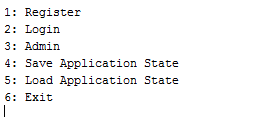
\includegraphics[width=60mm]{menuprincipal.png}
\caption{Menu inicial}
\end{figure}
\par Uma das funções mais básicas da aplicação baseia-se no registo e login de Utilizadores. No Menu inicial o utilizador tem
a opção de se registar ou então fazer login caso já possua uma conta.
\par Caso o utilizador deseje registar uma conta na aplicação terá de fornecer o seu e-mail, nome, password,
data de nascimento, a cidade e país de residência e o seu género (Masculino ou Feminino). A class \textbf{Main} invocará
os métodos necessários da classe \textbf{GeocachingPOO} que por sua vez invocará métodos da classe
\textbf{UserBase} para registar o utilizador.
\par Caso o utilizador especifique um e-mail já em uso será negado o registo da conta. Caso se verifique que o utilizador se
possa registar uma mensagem de sucesso aparecerá no ecrã, caso contrário uma mensagem de erro, informando o utilizador
o porquê da falha do registo.
\par Aproveitamos para implementar um método que encripta a password do utilizador para que deste modo, se um utilizador 
executar o método da classe \textbf{User} que permite obter a password apenas verá o resultado da encriptação. 
Sempre que é necessário confirmar se a password fornecida coincide com a guardada no utilizador o programar encripta a password fornecida e verifica se é igual ao resultado da encriptação já armazenado.\\
\begin{figure}[ht!]
\centering
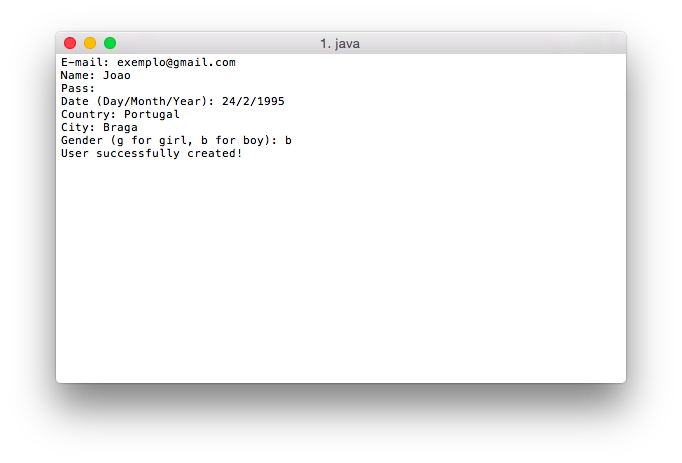
\includegraphics[width=100mm]{registo.png}
\caption{Registo de um utilizador}
\end{figure}
\\
\par Depois de um utilizador criar uma conta pode então executar o login, a classe \textbf{Main}, como trata de I/O, recebe qual
o e-mail e a password do utilizador, a classe \textbf{GeocachingPOO} trata do resto das invocações dos métodos necessários
para executar o login.
\par Caso o e-mail esteja associado a uma conta existente e a password fornecida confira com a password guardada então
será apresentado um menu ao utilizador, onde no topo lhe é apresentado o seu nome e o total de pontos que consegui juntar
até ao momento.
\par A partir deste menu de utilizador o utilizador consegue executar todas as funções básicas propostas, como, por exemplo,
mudar informações pessoais (nome, e-mail, género, password,..), criar uma cache de enter os 4 tipos que a aplicação
conhece, registar uma activadade, consultar as suas actividades, enviar pedidos de amizade, etc.
\par Decidimos também implementar uma opção no menu relativo a caches que permita a um utilizador descobrir quais as 
caches que se encontram a uma determinada distância (raio) de uma certa localização, indicada pelo utilizador. \\
\begin{figure}[ht!]
\centering
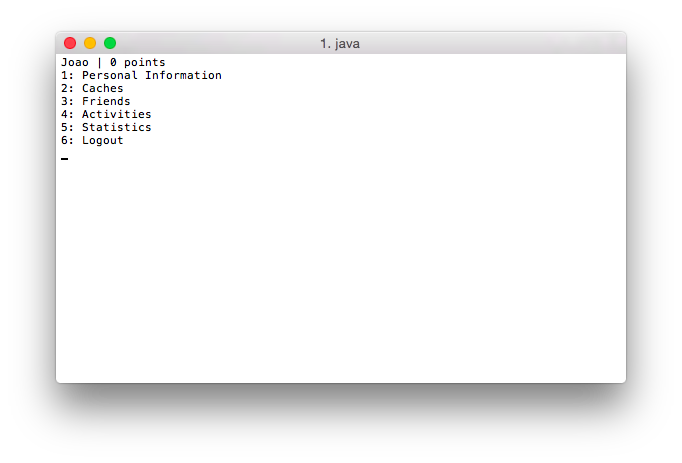
\includegraphics[width=100mm]{login.png}
\caption{Menu após o login}

\end{figure}
\begin{figure}[ht!]
\centering
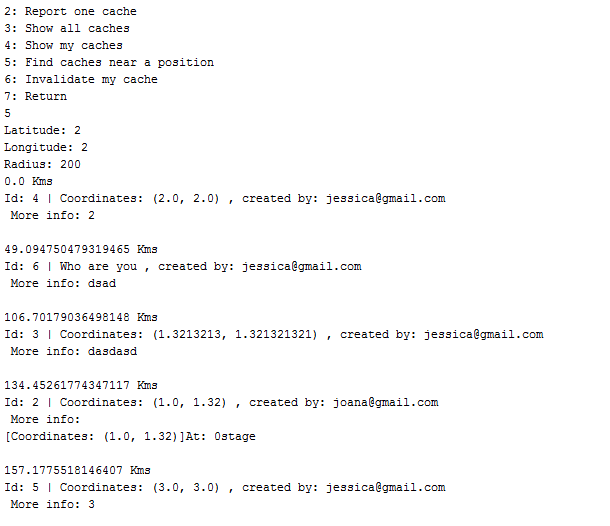
\includegraphics[width=90mm]{getNearCaches.png}
\caption{Encontrar caches perto de uma dada localização}
\end{figure}
\newpage
\section{Atividades e Estatísticas}

\subsection{Atividades}
\quad Quando o user encontra uma cache, regista uma nova Atividade que é automaticamente adicionada às Estatísticas.
\par Esta atividade têm como informações a data em que foi adicinada, a Cache que foi encontrada, os kilometros que foram percorridos para encontrar esta Cache, a pontuação ganha pelo feito e a Meteorologia desse dia.
\par O utilizador apenas tem de fornecer os dados quanto à Cache que encontrou e em que dia foi. O resto é tratado pelo programa, havendo simulações e cálculos.

\subsubsection{Quilómetros}
\quad  Quando adiciona a primeira atividade, são criadas as coordenadas iniciais do local onde o User iniciou a procura, geradas aleatóriamente fazendo cópia das coordenadas da Cache e um incremento da latitude e longitude de valores entre 0,001 e 0,4 por exemplo. No momento em que, ao adicionar esta primeira atividade, o programa calcula as distâncias entre estas coordenadas geradas aleatóriamente com base neste range, e as coordenadas da Cache, os kilometros calculados dão entre valores de 0,1km até 40 kms, em média.
Este incremento de latitude e longitude são métodos que usam o Math.Random, presentes na classe "Coordinates".
\par Caso já exista uma atividade anterior a esta que está prestes a ser adicionada, a distância calculada será entre as coordenadas desta cache e as coordenadas da cache da ultima atividade, tornando isto o mais realista possivel. A última atividade é a última posição conhecida do utilizador.
\\


\subsubsection{Meteorologia}
\quad  Na classe Meteo são geradas as meteorologias de uma forma aleatória também. Existem dois campos que dizem respeito à Temperatura e ao Estado de Tempo.
\par int Low = -10;
\par int High = 40;
\par São definidos os valores mínimos e máximos para a Temperatura. Para a Weather existem 7 tipos possíveis que são os seguintes:
\par Rainy 0
\par Stormy 1
\par Sunny 2
\par Cloudy 3
\par Windy 4
\par Foggy 5
\par Hail 6
\par A cada estado de tempo está associado um número que vai ser gerado aleatóriamente com o Math.Random entre os valores de inteiros de 0 até 7 (exclusive).
\\

\par Tudo isto é muito importante para as Estatísticas pois são calculados os pontos em cada Atividade, conforme o estado de tempo, os kilometros percorridos e o tipo de cache encontrada.
\par Para cada atividade existe um limite de pontos que decidimos atribuir: 100 pontos. Assim se quisermos diminuir ou aumentar este limite é só tratar da escala deste limite que será mais fácil. (Por exemplo, para cada atividade apenas querer 10 pontos, ou querer 1000, etc. ...).
\par Este limite de pontos total rege-se também por um limite às 3 atribuiçoes de pontos que criamos,  kilometros, meteorologia e cache, que são apresentados de seguida:
\begin{lstlisting}
private static int limit_points = 100;
private static int limit_points_cache = 50;
private static int limit_points_kms = 30;
private static int limit_points_meteo = 20;
\end{lstlisting}

\par * Decidimos atribuir mais pontos ao fator do tipo da cache. Se for uma Micro Cache atribuimos o mínimo de pontos (10) mas se for uma Mystery Cache o user consegue obter os 50 pontos máximos, dependendo também da dificuldade do Puzzle que foi atribuida. Como a estrela de dificuldade vai de 1 a 10, decidimos atribuir dificuldade * 5 pontos pela Mystery Cache.
\par Da mesma forma, tomamos decisões para o cálculo de pontos da Meteorologia e dos kilometros. Se percorrer mais kilómetros, ganha mais pontos e se o tempo estiver mau (Stormy, Hail ...) atribuimos o máximo de pontos para a Weather que são 10 pontos. Não esquecer que também temos a Temperatura, e para o caso de temperaturas extremas (muito baixas e muito altas) atribuimos também pontuações máximas. Depois, para cada situação à uma atribuição mediana conforme a meteorologia e temperatura.

TODO CODIGO A SER FEITO
\par O user tem possibilidade de visualizar as 10 últimas Atividades tanto dele como dos amigos, e de, se assim o quiser, as remover. Quando remove uma atividade, todas as informações e pontos adquiridos por esta são automaticamente retirados das estatisticas.


\subsection{Estatísticas}
\quad Quando às Estatísticas temos duas classes: StatisticYear e Statistic.
A razão pela qual temos duas classes é porque decidimos guardar também as Estatísticas Globais do user, ou seja, as estatísticas de todos os anos. Para melhor entender o funcionamento e a estrutura destas classes, começaremos por explicar a Statistic.

\par Na Statistic temos as estatísticas de um dado ano. A estrutura é a seguinte:
\begin{lstlisting}
ArrayList < TreeSet<Activity>>.
\end{lstlisting}

Tentamos criar um array para ter em cada indice o mês ligado ao conjunto de atividades desse mês mas é impossivel criar array com valores que não sejam primitivos, logo tivemos de mudar a estrutura para um ArrayList. Este ArrayList terá como indices o mês da estatistica. O seu conteúdo será o conjunto de Atividades realizadas nesse mês. Para adicionar uma atividade garantimos que não é possivel adicionar uma atividade se o ano não for o mesmo. Por isso é importante buscar o ano desta estatística, fazer set do ano desta estatística... O ano assumido como default é o current year que é 2015. Também são disponibilizadas funções como o de contar quantos tipos de cache num dado mês existem, e devolver num array, soma de pontos, de kms totais, numero de todas as caches encontradas, tanto para este ano como para um dado mês. Estas função são usadas como auxiliares na classe StatisticYear, e o porquê será entendido em seguida, quando for explicada a estrutuda da mesma.
\par StatisticYear é basicamente uma estrutura que mapeia um dado ano para uma Statistic. É esta a estrutura usada no programa pois facilmente se adiciona uma atividade nesta estrutuda, tendo o ano em que queremos inserir na data da atividade e usando os métodos existentes no Statistic como auxiliares. Todo o resto sobre o numero total de pontos, kilometros percorridos, numero de caches, etc... também são fornecidos por métodos de assinaturas iguais (tirando partido do Overloading), tanto para um dado ano como para todos os anos (global).


\par Permitimos ao user ver as suas estatiticas globais, anuais (de um dado ano) e mensais. Para as estatisticas mensais assumimos que ele quer ver um dado mês do current year (2015). Mas tal pode ser alterado facilmente, pedindo apenas mais uma informação extra ao user (que ano quer) antes de mostrar informações destas estatísticas.

\par Existe ainda uma opção para ver um gráfico de quantas caches dos tipos existentes o usuário encontrou, num dado mês.
\begin{figure}[ht!]
\centering
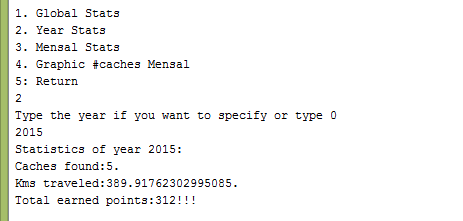
\includegraphics[width=90mm]{2015STATS.png}
\caption{Estatísticas anuais do ano 2015 de um utilizador}
\end{figure}
\begin{figure}[ht!]
\centering
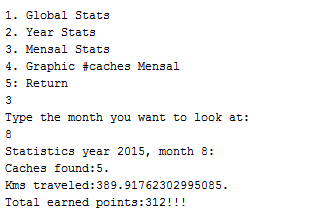
\includegraphics[width=90mm]{statsmes.png}
\caption{Exemplo de estatísticas de um dado mês}
\end{figure}

\pagebreak
\section{Amigos}
\par Implementamos também uma rede de amigos, cada instância de \textbf{NormalUser} contém variáveis para guardar
os IDs dos utilizadores que são seus amigos e os IDs dos utilizadores que enviaram pedidos de amizade.
Essas variáveis ficaram então definidas da seguinte forma:
\begin{lstlisting}[language=Java]
/* IDs dos amigos do utilizador */
ArrayList<Double> friends;
/* IDs dos utlizadores que enviaram pedidos de amizade */
ArrayList<Double> friend_requests;
\end{lstlisting}
\par A aplicação permite que utilizadores enviem pedidos de amizade a outros utilizadores inserindo o e-mail a quem desejam
enviar o pedido de amizade. O utilizador que recebe o pedido de amizade pode aceitar o pedido de amizade e ambos os
utilizadores guardam o ID um do outros na sua lista de amigos. A lista de amigos pode depois ser visualizada dentro da
própria aplicação.
\par Ao adicionar um amigo um utilizador poderá então, se desejar, visualizar a lista das 10 actividades mais recentes de qualquer um dos seus amigos.

\pagebreak
\section{Eventos}
TODO










\pagebreak
\section{Classes Main e GeocahingPOO}
\par Para poder utilizar as classes desenvolvidas para o projecto criamos uma class à parte, a classe \textbf{Main}, que contém
o método \em main. O único propósito desta classe é então lidar com a parte de I/O, relativamente apresentação de menus
e tratamento de input por parte do utilizador, esta classe também é responsável por invocar os diferentes métodos existentes
na classe \textbf{Geocaching} quando o utilizador necessitar de se registar, criar uma actividade, etc.
Também é neste método \em main que se lida com as Excepções criadas.
\par A classe \textbf{GeocachingPOO} contém variáveis das classes \textbf{CacheBase} e \textbf{UserBase} para poder guardar
os utilizadores e as caches criadas. Contêm também variáveis para guardar o utilizador ou administrador atualmente 'loggado'
e variáveis para controlo de IDs actuais a utilizar.
\par A classe contêm métodos para executar os vários requisitos do projecto, por exemplo, registar um utilizador novo, a classe
faz isto invocando métodos existentes em \textbf{UserBase}, já no caso de criação de caches, por exemplo, a classe invoca
métodos definidos em \textbf{CacheBase}. Basicamente a classe \textbf{GeocahingPOO} agrupa os vários métodos que sejam
precisos para utilizar a aplicação, definindo também quais os métodos necessários invocar para os diferentes objectos e ações
executadas.
\par Separar a parte de I/O da classe \textbf{GeocachingPOO} permite que a classe seja reutilizada noutros ambientes, por
exemplo com uma Interface Gráfica.

\pagebreak
\section{Salvaguarda do Estado}
\par Para guardar o estado da aplicação utilizamos classes já definidas em Java, nomeadamente a class
\textbf{ObjectOutputStream}. Utilizando esta classe é possível criar um ficheiro objecto com as informações de todos os
objectos da aplicação no estado actual. Para isso incluimos uma opção no menu principal que guardar o estado actual
da aplicação num ficheiro com o nome 'geocaching'.
\par Para carregar um estado anterior da aplicação utilizamos a class \textbf{ObjectInputStream} que permite ler objectos de
um ficherio objecto. Adicionamos uma opção no menu principal para carregar um estado anterior da aplicação, a aplicação
tenta automaticamente ler o ficheiro 'geocahing' criado quando se guardar o estado da aplicação, caso o ficheiro não esteja
na mesma diretoria onde se executa a aplicação o estado anterior não será carregado.

\pagebreak
\section{Tratamento de Excepções}
\quad Decidimos colocar todas as excepções num package chamado Exceptions para uma melhor visualização das classes e
clareza no diagrama. Para todas as classes que implementam Excepções é feito import deste Package. Apenas a função
\em main faz o tratamento de Excepções.
\pagebreak
\section{Conclusão}




\end{document}
